\documentclass{article}

\usepackage[inline]{enumitem}

\usepackage{url}
\usepackage{graphicx}
\graphicspath{ {./figures/} }
\usepackage{amsfonts}% to get the \mathbb alphabet
\usepackage{booktabs}
\usepackage{multirow}


\title{Decentralised Mining Pool for Bitcoin (Draft 0.1)}
\author{Kulpreet Singh}
\date{}

\begin{document}

\maketitle

\begin{abstract}
  Bitcoin p2pool's usage has steadily declined over the years,
  negatively impacting bitcoin's decentralisation. The primary
  problems with p2pool are twofold. First, the variance in earnings
  for miners increases with total hashrate participating in the
  pool. Second, payouts to miners require a linearly increasing
  blockspace with the number of miners participaating in the
  pool. Building a directed acyclic graph (DAG) of miner's shares and
  the use of payment channels are two proposals trying to alleviate
  these problems. In this paper, we present a unified solution that
  uses a DAG to track miners shares and uses payments channels to
  reward miners. The shares calculation is verified by all
  participants of the pool, and the rewards are paid out by an
  anonymous hub communicating with the miners using I2P. Using the
  payment channels construction, neither the hub nor the miners can
  cheat. We show that our approach is incentives compatible and
  describe how the hub maintains its anonymity to resist DDoS attacks.
\end{abstract}
   
\section{Motivation}

P2Pool~\cite{p2pool:wiki} helps bitcoin's decentralisation by allowing
miners to select which transactions they mine. This avoids any
potential transaction censorship by pool operators. However, the
construction used by P2Pool faces a number of problems that resulted
in miners abandoning the pool. The most often cited problems are:

\begin{enumerate}
\item Large variance in earnings for miners.
\item Large number of stale blocks.
\item Large block space requirement for payouts.
\end{enumerate}

The first two problems are a direct consequence of the shares block
rate limited to 30 seconds for the bitcoin p2pool. Intuitively, with
only one block possible every thirty seconds, increase in the hashrate
on P2Pool results in shares competing to be the next block in the
p2pool chain. Where only one winning share will be rewarded for its
PoW, and the others have to rue their bad luck. An increase in the
share rate results in even more stale blocks. With miners not rewarded
for stale blocks, it leads to increase in the variance of the miner
rewards~\cite{mcelrath:variance}. Ethereum's inclusive
protocols~\cite{inclusive-protocols} help alleviate the problem for
the Ethereum blockchain where smaller pools can continue to get
rewarded for their PoW, without an increase in variance with
increasing in global hash rate.

Knowing the challenges faced by P2Pool, we list the goals of a new
decentralised mining pool as:

\begin{enumerate}
\item Reduced variance for miners with increasing pool hash rate.
\item Payouts for miners with constant size block space requirement.
\item Independent miners can build their own blocks.
\item Provide building blocks for a hash rate futures
  market.~\footnote{We don't elaborate on this goal in this paper, but
    readers can look up the gist on TerraHash coins
    https://gist.github.com/kulpreet/19927c7188a4224ce2de43efb3c69370}
\end{enumerate}

\section{Current Proposals}

TerraHash Coin~\cite{mcelrath:variance}, Jute~\cite{jute}
and~\cite{spectre} are some of the attempts to use a DAG for faster
block times. However, they focus on changing the consensus layer of
bitcoin. These proposals allow for miners to produce shares that have
conflicting transactions and then apply rules to find a set of
transactions acceptable at various cuts of the DAG.\@

Belcher~\cite{channels-for-rewards} proposes using payment channels as
to avoid using block space for making payouts to miners. The
construction uses payment channels between federated hubs to pay
miners after a block has been successfully mined. The payouts are made
after a long enough period, similar to the 100 blocks requirements for
spending from coinbase transactions. Miners register with hubs where
bitcoin has been locked in to open payment channels to miners. The
construction shows how both miners and hubs can not cheat and how the
funders of the hub can earn a reward for funding the payment channels.

The two ideas of using a DAG and payment channels for rewards
payouts together present a potential path for rebooting P2Pool. In the
rest of the paper we present a modified version of TerraHash Coin and
show how the various components work together.

\section{Decentralised Bitcoin Mining}

In this section we present a modified version of TerraHash Coin. We
propose building a DAG of miner's shares and use that to determine the
payout distribution between miners. We then show that the payout
distribution rewards miners for the shares they find and broadcast to
the p2p network in a timely manner.

\subsection{A DAG of Shares}

Braiding the blockchain proposal~\cite{mcelrath:variance} shows how
smaller more frequent blocks can form a directed acyclic graph (DAG)
of blocks, with each block pointing to one or more one previous
blocks. Blocks in the braid, called beads, can have transactions
repeated in different blocks. The proposal describes how duplicate and
double spend transactions can be resolved to reach a decision on the
state of the ledger at any cut of the DAG.\@

In the proposal, miners a coin native to the braid blockchain, called
TerraHash Coin. This coin can then be swapped for Bitcoin. The
proposal doesn't yet define how this native coin will be swapped for
bitcoin. Some of the suggestions under discussion include using atomic
swaps, burning the TerraHash Coin, or using financial instruments like
futures of the bitcoin's hash rate to swap TerraHash Coins for BTC.\
The problems with the atomic swap approach is the need for $O(n)$
block space in number of miners, as we need two transactions to
execute a swap with each miner. Burning THCoins for BTC requires a
trusted third party to execute this. Finally, trading THCoins for BTC
futures has the problem of introducing centralisation on the futures
market operator. There is some discussion around using DEXes for
executing futures contracts, but and we don't go down that route here.

We propose taking a modified approach, where the blocks of a DAG
represent shares of the mining pool. Miners broadcast their shares to
the network using a gossip protocol and all the miners maintain the
DAG as a replicated database. This DAG can be pruned to the bitcoin
block height that miners have received payouts for. Shares broadcast
by miners include a hash pointer to all previous shares received from
other miners, this ensures the DAG is eventually consistent on all p2p
participants.

\subsubsection{Building Blocks}\label{sec:building-blocks}

Each miner builds their own block, selecting transactions according to
their own criteria. We call this block the \textsc{work}. The
description of \textsc{work} is then disseminated to the p2p network
of miners using the compact block
specifications~\cite{compact-blocks}.

The miner then starts mining on \textsc{work} and generates
\textsc{share}s. Each \textsc{share} is mined at a difficulty level
chosen by the miner. This difficulty can be dynamically chosen by the
miner after each \textsc{share}, depending on miner's observation of
the p2p network's hashrate. This dynamic adjustment allows miners to
adjust the rate at which they produce \textsc{share}s.

Figure~\ref{fig:work-share} shows the relationship between
\textsc{work} and its \textsc{share}s. Each \textsc{work} created by a
miner can result in multiple \textsc{share}s and both the
\textsc{work} and \textsc{share}s are broadcast to the p2p
network. When a miner receives a \textsc{work} from other miners it
validates this \textsc{work} using a local bitcoin node. When a
\textsc{share} is received by a miner they are validated against the
most received \textsc{work} from the miner.

\begin{figure}
  \begin{center}
    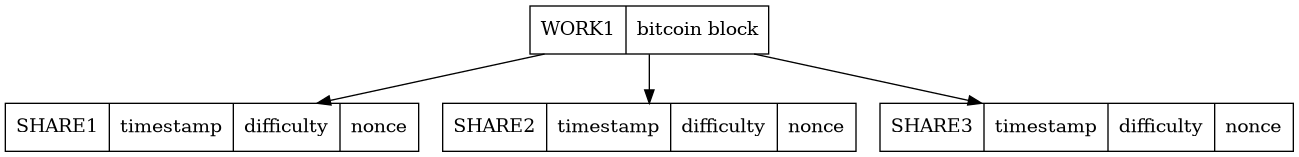
\includegraphics[width=1.0\textwidth]{work-share}
    \caption{Each \textsc{work} generated and shared by a miner is then
      followed by the \textsc{share}s the miner finds.}\label{fig:work-share}
    \end{center}
\end{figure}

The nodes in the DAG are \textsc{share}s mined at varied difficulty
levels. Each \textsc{share} that matches or exceeds the current
bitcoin difficulty starts a new $epoch$ for the p2p mining
pool. Figure~\ref{fig:epoch} shows $l$ and $r$ as the two valid
bitcoin blocks that have been mined such that they meet bitcoin's
difficulty at the time, and all the blocks between $l$ and $r$ are in
the same $epoch$.

\begin{figure}
  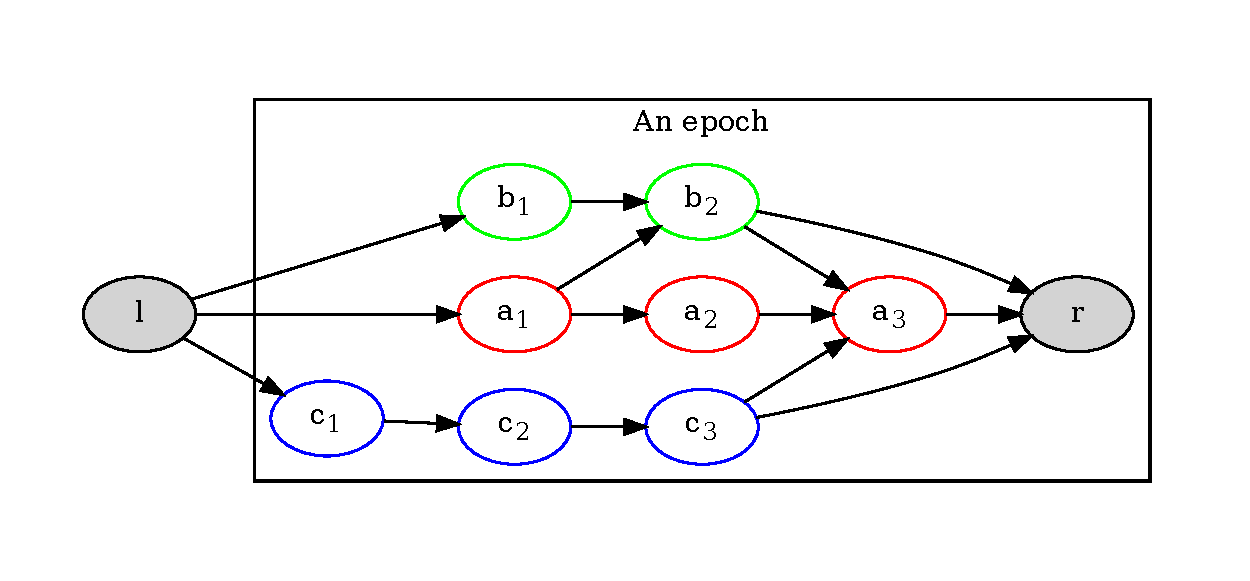
\includegraphics[width=1.0\textwidth]{epoch}
  \caption{A epoch is defined as all the \textsc{share}s mined between two
    bitcoin blocks. Here all the \textsc{share}s between $l$ and $r$ are in
    the same $epoch$.}\label{fig:epoch}
\end{figure}

When a miner starts working on a \textsc{share} it includes a
reference to the most recent \textsc{share} from all other miners that
the miner has received valid shares from. Note, the miner also has
access to \textsc{work} blocks from all participating miners. If a
miner doesn't have the \textsc{work} block from another miner, then it
rejects any \textsc{share}s received from the other miner.

In the next section we then describe how all peers compute their fair
share of profits using the DAG of shares. We then show how our reward
computation algorithm is incentives
compatible as per~\cite{incentives-compatible}.

%% - block datastructure
%%   - coinbase reward goes to Hub's address
%%   - ignore this for now, we'll show how the reward is distributed in a
%%     trustless manner to all miners.
%% - DAG of shares
%%   - Epochs: start from and end with bitcoin block
%%   - Epoch ends when a valid bitcoin block with current bitcoin
%%     difficulty is found
%%   - Immediately send mined bitcoin block to bitcoin network
%%   - Hub will distribute the reward in around 100 blocks time
%% - Use compact blocks to inform others about the block we are mining
%%   - Other miners can decide to include your block as a previous block
%%     or not, whenever we find a solution and announce it.
%%   - We need to model the network traffic and latency
%% - Keep mining the same block, until end of epoch
%%   - For each block mined, share the solution with p2p network
%%   - Only if the mined block meets the current bitcoin difficulty
  
  
\subsection{Incentives Compatible Rewards}\label{sec:rewards}

Each participating node, which includes the miners and the hub,
maintains a local replica of the the \textsc{share}s DAG.\@ Each
\textsc{share} includes a reference to the shares the miner was aware
of when the \textsc{share} was found. If a miner $a$ doesn't include
the \textsc{share}s of miner $b$, it signals a failure of
communication between the two miners. We introduce a rule that miner
$a$ in such a situation stops including references to $b$'s
\textsc{share}s.

The incentive in lay terms is that all miners should honestly include
the \textsc{share}s discovered by other miners, as otherwise they will
most likely be excluded by other miners and they will lose the
opportunity to be rewarded for their work. We identify this
degenerative case of ``isolated miners'' and argue that miners have no
incentives to act in this manner. Figure~\ref{fig:isolated-miners}
shows a DAG where all three miners $a$, $b$ and $c$ are working
independently. In such a situation when the miner $a$ discovers a
share $a_3$ that is a valid bitcoin block and the reward is not shared
with any other miner as $a_3$ does not include any references to
shares from other miners.

\begin{figure}
  \begin{center}
    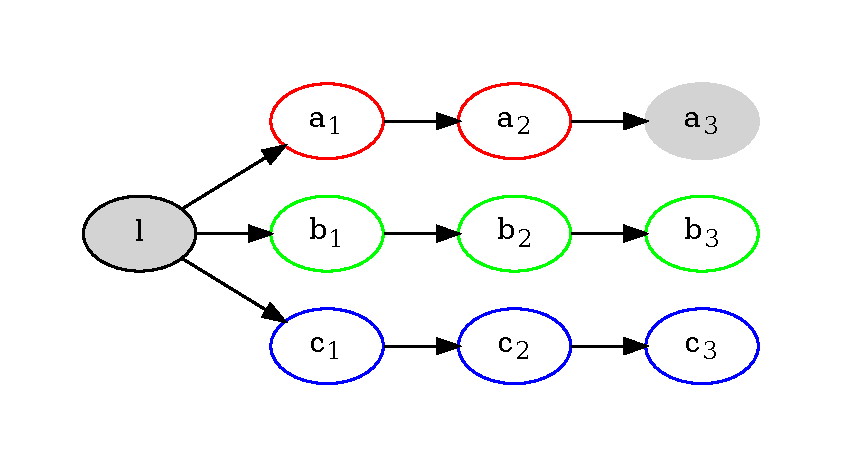
\includegraphics[width=0.65\textwidth]{isolated-miners}
    \caption{$a$ discovers a share and the reward is not shared with any
      other miner.}\label{fig:isolated-miners}
  \end{center}    
\end{figure}

With the above understanding of why miners will co-operate, we now
state the rules to calculate how the block reward should be divided
between miners.

\begin{enumerate}
\item Traverse the DAG in reverse order from the \textsc{share} that
  found a bitcoin block to the previous bitcoin block found and
  collect this set of shares.
\item From the above set of shares remove all shares that don't have
  a reverse path to the previous bitcoin block.
\item Distribute the reward between miners weighted by the sum of
  the difficultly of all \textsc{share}s found by miners.
\end{enumerate}

As an example, consider the p2p network of miners $a$, $b$ and $c$
with the DAG of shares as shown in Figure~\ref{fig:shares-dag}. In the
DAG, the set of shares that receive reward proportional to their
difficulty are $\{a_1..a_5, b_1..b_3\}$. The shares $\{c_1..c_3\}$ do
not receive any reward as they are not reachable from the bitcoin
block, $a_5$, even if they are reachable from $l$.

For the second bitcoin block $b_5$ only the miners $a$ and $b$ receive
rewards in proportion to the difficulties of their shares
$\{b_4, b_5, a_6\}$. $c$ doesn't receive any reward for $c_4$ as it is
doesn't include a reference to the last found bitcoin block $a_5$.

\begin{figure}
  \begin{center}
    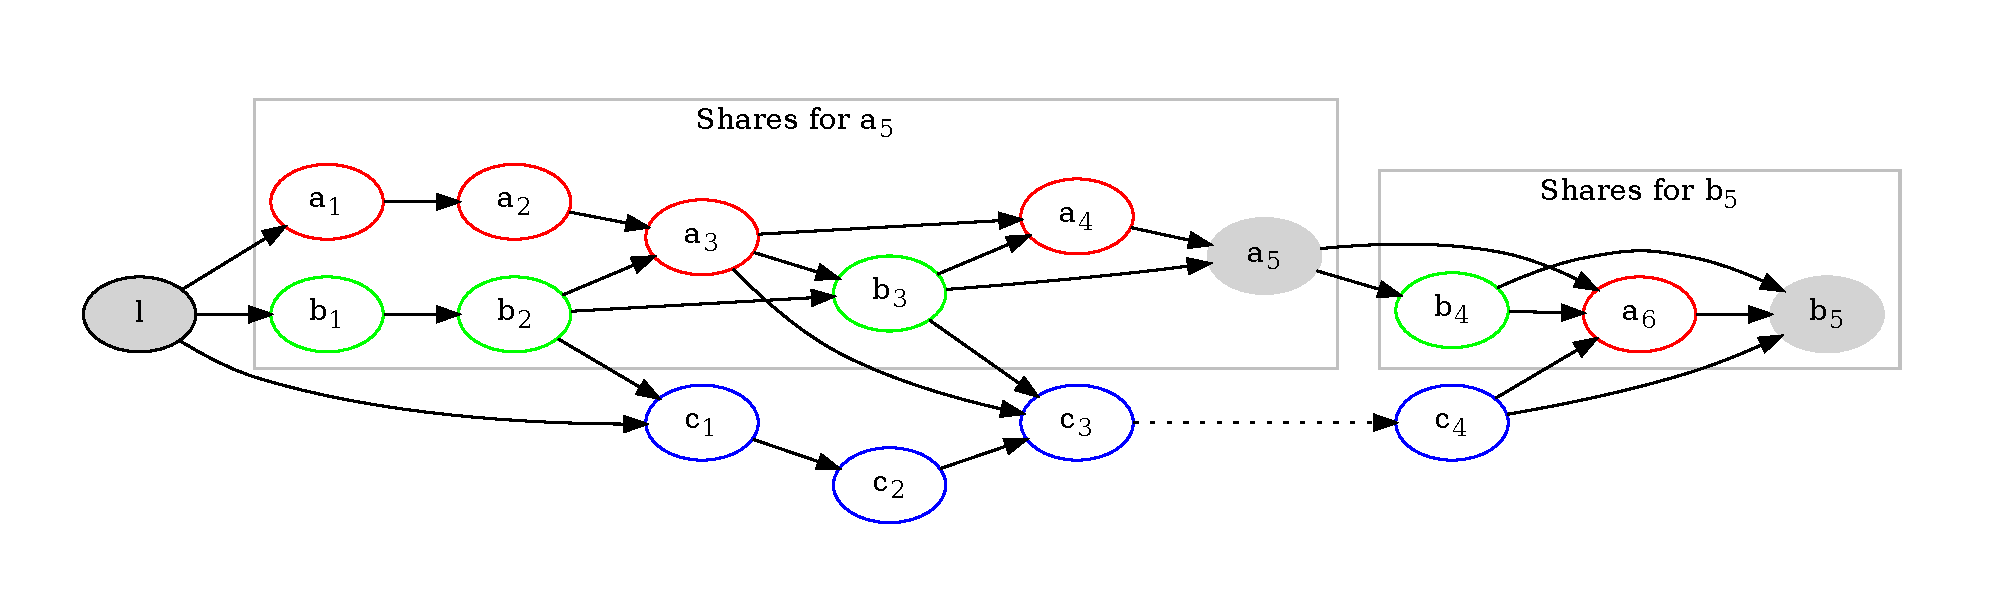
\includegraphics[width=1.0\textwidth]{shares-dag}
    \caption{Two epochs in a DAG of shares mined by three mines ---
      $a$, $b$ and $c$. The shares in grey meet the bitcoin difficulty
      at the time they were mined.}\label{fig:shares-dag}
  \end{center}
\end{figure}

Given the above rules, we show how they together provide an incentives
compatible reward function~\cite{incentives-compatible}. We present an
outline of proofs that will be be formalised in future work.

\subsubsection{Incentive Compatibility}\label{sec:incentive-compatability}

A reward function is incentive compatible when every miner's best
response strategy reports full solutions
immediately~\cite{incentives-compatible}. Where a ``full solution'' is
a share that meets the bitcoin network's difficulty requirement.

Given the rules in Section~\ref{sec:rewards}, if a miner finds a
bitcoin block the miner wants to get maximum reward possible based on
all the shares it has found and therefore is incentivized to announce
their \textsc{share} as soon as it finds the block. The longer a miner
doesn't announce the bitcoin block to the bitcoin network, the higher
the probability that some other miner on the pool will find a
different bitcoin block that doesn't reward their latest shares that
haven't reached the other miner. Further still, the rewards
calculation can be adjusted to give an extra reward to the miner that
finds the block. This is similar to what p2pool does and Belcher also
mentions in his proposal.

\subsubsection{Proportional Payments}\label{sec:proportional-payments}

As per~\cite{incentives-compatible}, we require that miners are paid
in proportion to the amount of work they have performed.

Since rewards are calculated at the end of an epoch and a miner is
incentivized to include hash pointers to the most recent shares seen
from all miners, it directly follows that all miners are guaranteed
payments for their shares that have reached the miner who found the
block. It is also clear here that miners are incentivized to propagate
their shares to the network as fast as they can.

\subsubsection{Budget Balanced}\label{sec:budget-balanced}

Again, as per~\cite{incentives-compatible} we would like the pool
operator to never incur a deficit. From the rules, since rewards are
paid at the end of the epoch, a hub pays out rewards without losing or
retaining any amount.

\subsection{Payment Channels}\label{ref:channels}

We propose using Payment Channels for paying miners based on the work
by Belcher~\cite{channels-for-rewards}. The construction of the
payments channels we present is similar to Belcher's construction, but
there are a few changes and we highlight them before describing the
details.

\begin{itemize}
\item In the Belcher proposal, the pool had to predict how much work
  miners will be able to contribute for the next block. Instead our
  DAG based scheme results in an incentives compatible distribution of
  rewards among miners.
\item Belcher proposes uses multiple hubs to percent DDoS attacks on
  hubs, we instead use a single hub, and prevent DDoS attacks by keeping the
  hub hidden using I2P~\cite{i2p, i2p-censorship-resistance} for
  communication between the hub and miners.
\end{itemize}

The rest of the construction is the same as presented by Belcher ---
There is a one-way channel between the hub and each of the miners. The
hub updates the state of each channel with appropriate reward after
each block is found.

% TODO
% Question: How do we know the Hub is not creating coinbases with
% different preimages with each miner?

% Answer: Miners receive the pubkey for all other miners with the
% \textsc{work} announcement. Using this and the structure of the
% coinbase transactions, miners validate that the coinbase matches the
% hub's preimage, and the miner's pubkey.

\subsubsection{Coinbase}

We use Belcher~\cite{channels-for-rewards} construction where each
miner builds a coinbase transaction that can be spent in one of the
following three ways:

\begin{enumerate}
\item Co-operatively by Hub and Miner, or
\item By the Hub with a hash lock for pre-image \verb|X|, or
\item By the Miner that found the bitcoin block, but after waiting for
  six months.
\end{enumerate}

\begin{table}
  \centering
  \begin{tabular}{ lr }
    \bfseries Coinbase \\
    \midrule
    \verb|2 H M 2 CHECKMULTISIG| & $(cb_1)$ \\
    \verb|OR| \\
    \verb|hash(X) + Hub P2WPKH| & $(cb_2)$ \\
    \verb|OR| \\
    \verb|M and CHECKSEQUENCEVERIFY 6 months| & $(cb_3)$\\ 
    \midrule
  \end{tabular}
  \caption{Coinbase transaction with hub and miner public keys.}\label{table:coinbase}
\end{table}

The scriptPubKey for the above conditions in the coinbase is shown in
Table~\ref{table:coinbase}. These conditions mean that the hub can not
spend the coinbase without revealing the pre-image $X$. This pre-image
is included in the construction of payment channels, as we will see in
the next section. This use of pre-image in both the coinbase and the
payment channel definition guarantees that miners get paid for their
accumulated payouts if the Hub defects and spends through the $cb_2$
branch. We discuss how the miner and the hub don't gain by defecting
in Section~\ref{ref:defecting}.

\subsubsection{One-way Channels}

One-Way payment channels between hub and all miners allow miners to
receive payouts while consuming a constant size blockspace in the
bitcoin block they mine. The use of payment channels is what makes
braidpool scale up without losing blockspace. Braidpool thus avoids
losing the fees that can be earned from the blockspace.

Just like in the early versions of proposal by Belcher we use one-way
payment channels. One-Way payment channels solve the problem of
aggregating a miner's payouts requiring a single blockchain
transaction for spending multiple payouts earned from their PoW
shares.

We use one-way instead of bidirectional payment channels as an initial
implementation for Braidpool. If required we can switch to
bidirectional channels~\cite{poon2016bitcoin} allowing miners to spend
their mining payouts over the lightning network. However, for now, we
deliberately stay away from the complexity of making the hub a
lightning node. If there is interest from miners to use the lightning
network, we can build in the future.

Each miner has a one-way payment channel with the hub using a two of
two multisig with a time lock of six months. For each payout a miner
receives over the payment channel, the hub will charge an agreed upon
fees between the miner and the hub. Belcher's proposal recommends a
$0.1\%$ fees for the hub.

\subsubsection{Payment Channel Transactions}

The hub creates a funding channel locking an amount $R$ of
bitcoin. The miner then creates a refund transaction, spending the
funding transaction and sending the $R$ bitcoin back to the hub. The
refund transaction has a locktime of six months allowing the miner to
accumulate their payout over the six month period. The protocol can be
extended to allow each miner to agree upon a locktime with the hub. In
this case, the trade-off will be between the fees charged by the hub
and the length of the locktime.

The funding transaction includes an input from the hub and an output
that can be spent in one of the two conditions shown in
Table~\ref{fund-tx}. \verb|H| and \verb|M| are the public keys for hub
and miner, they are called the co-operative keys by Belcher. While
\verb|H'| and \verb|M'| are alternative public keys for hub and miner,
and are called the uncooperative keys in the Belcher proposal.


\begin{table}
  \centering
  \begin{tabular}{ llr }
    \multicolumn{2}{c}{\bfseries Fund Transaction} \\
    \midrule
    \bfseries Input & \bfseries Output \\
    \midrule
    Hub's UTXO & \verb|2 H  M  2 CHECKMULTISIG| & $(f_1)$ \\
    (Signed by the hub) & \verb|OR| \\
                    & \verb|2 H' M' 2 CHECKMULTISIG + Hash(X)| & $(f_2)$ \\
    & (R coins) \\
    \midrule
  \end{tabular}
  \caption{Fund transaction for payment channel between hub and miner.}\label{fund-tx}
\end{table}


The hub doesn't broadcast the funding transaction, instead it waits
for the miner to create refund transaction. This is the same as any
other timelocked one-way channel construction, i.e.\ the miner creates
a refund transaction with a timelock, signs it and sends it to the
hub. The refund transaction is shown in Table~\ref{refund-tx}.

\begin{table}
  \centering
  \begin{tabular}{ ll }
    \multicolumn{2}{c}{\bfseries Refund Transaction. Locktime 6 months} \\
    \midrule
    \bfseries Input & \bfseries Output \\
    \midrule
    Fund Tx & \verb|P2WPKH Hub's address| \\
    (Signed by miner) & (R coins) \\
    \midrule
  \end{tabular}
  \caption{Refund transaction signed by miner and held by
    hub.}\label{refund-tx}
\end{table}

With the refund transaction, if the miner stops responding, the hub
can get a refund in six months time. However, the hub can be attacked
by sending requests to open new channels and locking up the hub's
liquidity. The hub responds to a miner's channel open request only
after the miner has contributed enough shares. This could be a
parameter of the pool instantiation, anywhere between one to 100
bitcoin blocks. The threshold number of shares required before opening
the channel is a configuration parameter for the hub. The miner will
still receive the payouts for the shares generated, it is only that
the channel opening is delayed.

On receiving the refund transaction, the hub broadcasts the funding
transaction. Once the funding transaction is confirmed, the hub can
start sending payouts to the miner. These payouts are determined in
proportion to the shares found by the miner and included in the DAG as
described in Section~\ref{sec:rewards}.

The payment transactions are updates to the channel where each update
increases the earnings of the miner. The payment transactions are
signed by the hub using the non-cooperating key, \verb|H'|.
Table~\ref{payment-transaction} shows the structure of the payment
transactions.

\begin{table}
  \centering
  \begin{tabular}{ llr }
    \multicolumn{2}{c}{\bfseries Payment Transaction} \\
    \midrule
    \bfseries Input & \bfseries Output \\
    \midrule
    Fund Tx & \verb|2 H  M  2 CHECKMULTISIG| & $(p_1)$ \\
    (Signed by the hub using H') & \verb|OR| \\
                    & \verb|2 H' M' 2 CHECKMULTISIG + Hash(X)| \\
                    & (Hub: $R - earnings$; Miner: $earnings$) & $(p_2)$\\
    \midrule
  \end{tabular}
  \caption{Payment channel update transaction sent from hub to the
    miner.}\label{payment-transaction}
\end{table}

The hub updates the payment channel for each miner with payouts as
determined by the incentives compatible rewards algorithm shown in
Section~\ref{sec:rewards}. In the next section we present how the
payouts are distributed, we then show how the hub and the miners are
dis-incentivized to cheat.

\subsection{Anonymous Payouts}

Once a miner mines a share that also meets the currently bitcoin
difficulty, the miner immediately broadcasts the block to the bitcoin
network. The coinbase of this block as shown in
Table~\ref{table:coinbase} can now be spent by

\begin{description}
\item[Co-operative Branch:] The miner and the hub by both signing the
  first branch co-operatively.
\item[Hub Branch:] The hub alone, by publishing the pre-image \verb|X|.
\item[Miner Branch:] the miner alone, after waiting for six months.
\end{description}

The proposal by Belcher specifies a payout algorithm that requires the
hub updates the state of all channels, i.e.\ make payment to all
miners. Once it has done so, the miner signs the first branch of the
coinbase transaction and hands the coinbase to the hub. The hub can
now redeem the entire payout. We use the same approach, requiring the
miner to receive all channel updates from the hub before signing the
co-operative branch. The miner first verifies that that the channel
updates are properly signed by the hub, and there is one update for
all miners in proportion to the rewards distribution algorithm.

\subsection{Defecting Does Not Pay}\label{ref:defecting}

Using the above construction of the payment channel and the
distributed payout algorithm, we now show that defecting by the hub or
the miner doesn't pay.

\subsubsection{Hub Defects}\label{ref:hub-defects}

If the hub defects and pays itself from the coinbase it uses the
$cb_2$ branch of the coinbase. In doing so, the hub has to reveal the
pre-image \verb|X|. With the pre-image available, all miners will use
the $p_2$ branch of their payment channel transactions and close their
channels and receive all payouts earned up to that block.

It is possible that the hub defects on the very first block mined and
the miners lose their earnings for that single block. But that will
end the pool before it could be useful.

The hub could defect after a few blocks have been mined. In such a
case the miners will receive their fair share of earnings for all
previous blocks, but it will again be the end of life for the pool.

Remember the hub charges fees to fund the payment channels between the
itself and the miners. When the pool ends, the hub loses a profit
making opportunity. We argue that the incentive to defect reduces as
the size of the pool grows.

It is worth noting that if the hub is co-opted, all it can do is deny
miners a payouts for the number of blocks the pool delays the payments
by. We introduced the idea of this ranging from one to 100
blocks. Further, if the hub is co-opted, all miners will immediately
close their channels, collect their payouts and re-organise with a
different hub.

\subsubsection{Miner Defects}\label{ref:miner-defects}

A miner that found the block could chose to not sign the co-operative
branch of the coinbase. In such a case, the hub will wait for a
timeout period much shorter than the locktime on the miner
branch. This will close all channels and require that all these
channels are opened again. Such an attack by the miner will hurt
miners on the network who have not yet earned enough payouts to
amortise the cost of closing the channel.

Say a miner starts participating in the pool, and after $N$ blocks
successfully mines a bitcoin block, but refuses to sign the
co-operative branch of the coinbase allowing the hub to claim the
coinbase reward. In such a case all miners have to close their
channels and claim the rewards they have earned. Miners who recently
joined the pool stand to lose the most because of the forced closure
of channels.

However, the miner also loses any payouts for all the shares it mined
since the last block was found by the pool. A malicious miner could
contribute a large portion of the pool's hash rate and then refuse to
sign the co-operative branch. This will disrupt the functioning of the
pool and the censor could be willing to execute such an attack. The
only defence here is that the miners re-organise and start a different
instance of the pool hiding their activity behind I2P tunnels. We
elaborate on our use of I2P in
Section~\ref{sec:hub-miner-communication}.

\subsubsection{Hub and Miner Collude}\label{ref:collusion}

The hub and the miner could collude where they co-operate to spend the
coinbase to themselves without requiring that the hub pays all other
miners as per the reward schedule. The motivation for the miner is
clear that it earns a big payout, however, such an action by the hub
will end the pool and the stream of future profits for the hub.

%% \subsubsection{Miner Sybil Attack}\label{ref:sybil-attack}

\subsubsection{DDoS on the Hub}\label{ref:ddos-attack}

The hub can be attacked using a distributed denial of service attack
rendering it unable to process requests to open new channels and to
distributed payouts to miners. Belcher in his proposal suggested the
use of multiple hubs as a defence against such an attack. The proposal
also points out that multiple hubs will reduce the liquidity required
to open channels with miners.

According to Belcher's proposal, with multiple hubs available on the
p2p network miners will open channels to all hubs and receive payouts
from all of the hubs. The coinbase is split between hubs in such a way
that if any hub defects, the other hubs can still spend the coinbase
and split the block reward between them. In this way all miners
receive payouts in proportion to the shares contributed by them.

Creating a larger coinbase for multiple hubs scales if we can use
Taproot~\cite{bip340,bip341, bip342} once it is activated. The
solution uses staggered timeouts for hubs to spend the coinbase in
case of hubs defecting or coming under DDoS attacks. This option is
worth exploring once Taproot is enabled and the pool will benefit from
multiple hubs. This will be even more useful as with the multiple hubs
construction reduces the liquidity requirements for all hubs. The only
problem is that in case of hubs defecting, the staggered timeouts can
result in a large wait for the payouts to be distributed.

We propose a different solution that requires a single hub. The
advantage is a simpler channel construction and allow us to build the
mining pool without waiting for Taproot activation. The single hub
approach requires that all miners open I2P tunnels to gateways and
publish the gateway's address in the shares they broadcast on the p2p
network. The hub then can communicate with miners by opening new
tunnels and remaining anonymous. We present this approach in the next
section.

\subsection{Anonymous Hub Miner
  Communication}\label{sec:hub-miner-communication}

The hub and the miner need to exchange messages at the time of channel
creation as well updating the channel state when the hub makes a
payout to the miners. The channel management messages are exchanged
infrequently as compared to the \textsc{share}s broadcast messages and
don't have the same timeliness requirements as the shares
broadcasts. We propose adopting a solution that doesn't compromise on
the hub's anonymity and makes a trade-off with increased latency of
the channel management messages.

We use I2P's tunnels to avoid compromising the anonymity of the hub
I2P works by setting up separate inbound and outbound
tunnels. According to the I2P documentation~\cite{i2p-tech-intro}:

\begin{quote}
  A tunnel is a directed path through an explicitly selected list of
  routers. Layered encryption is used, so each of the routers can only
  decrypt a single layer. The decrypted information contains the IP of
  the next router, along with the encrypted information to be
  forwarded. Each tunnel has a starting point (the first router, also
  known as ``gateway'') and an end point. Messages can be sent only in
  one way. To send messages back, another tunnel is required.
\end{quote}

\begin{figure}
  \begin{center}
    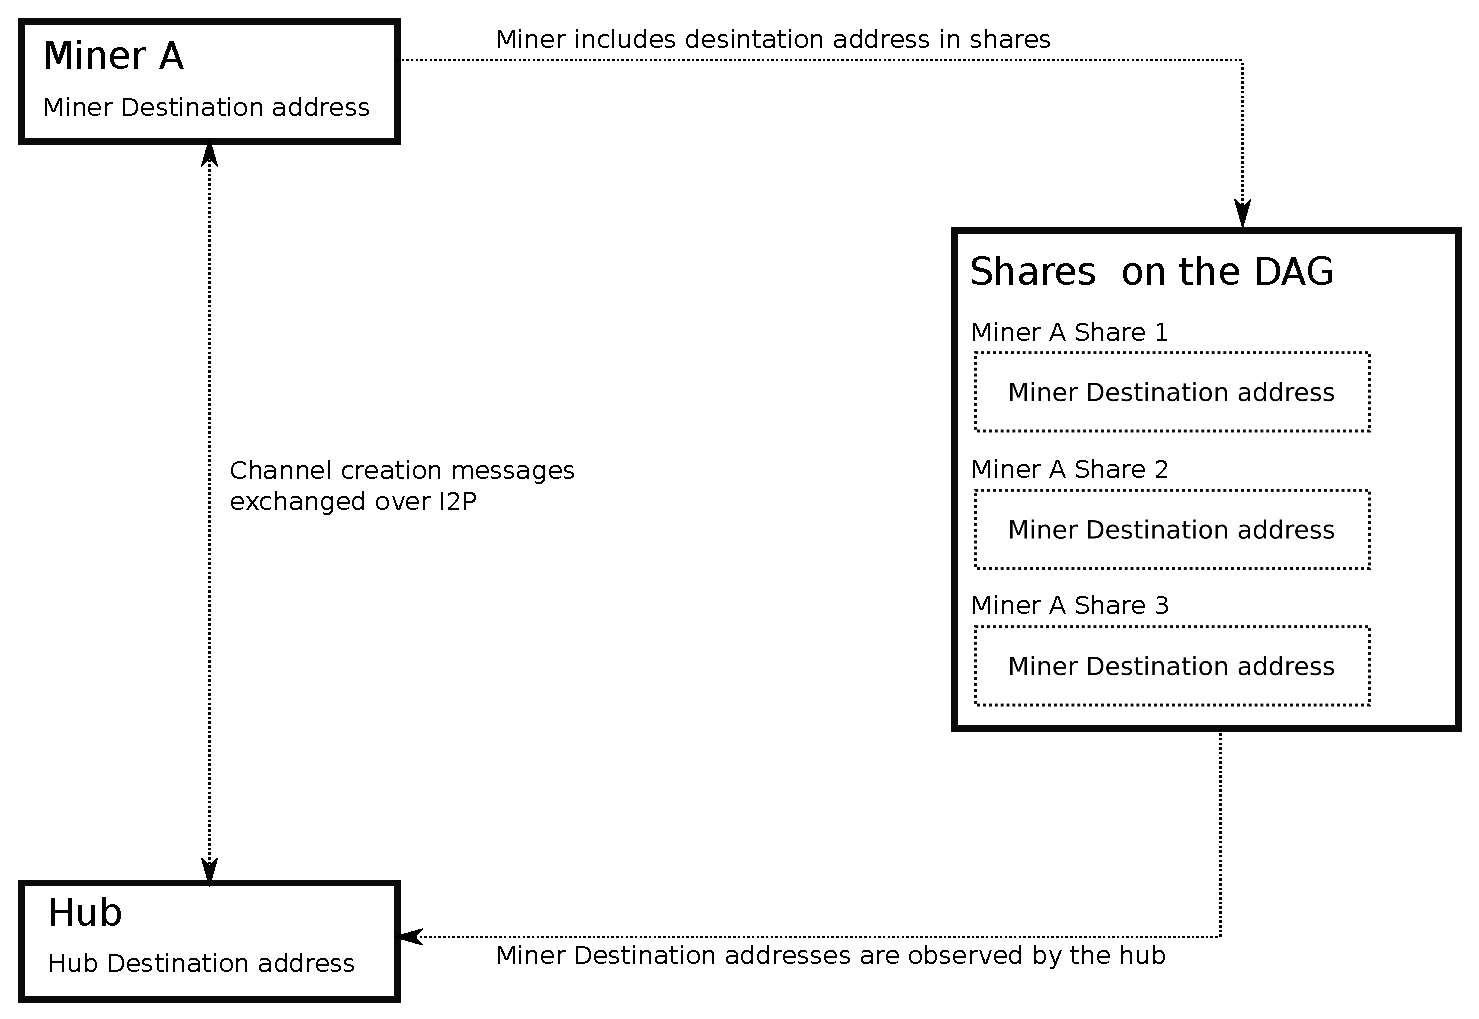
\includegraphics[width=0.75\textwidth]{new-miner-communication.eps}
    \caption{Discovery of miner I2P destination addresses enables
      communication for creating channels.}\label{fig:new-miner-communication}
  \end{center}
\end{figure}

\begin{figure}
  \begin{center}
    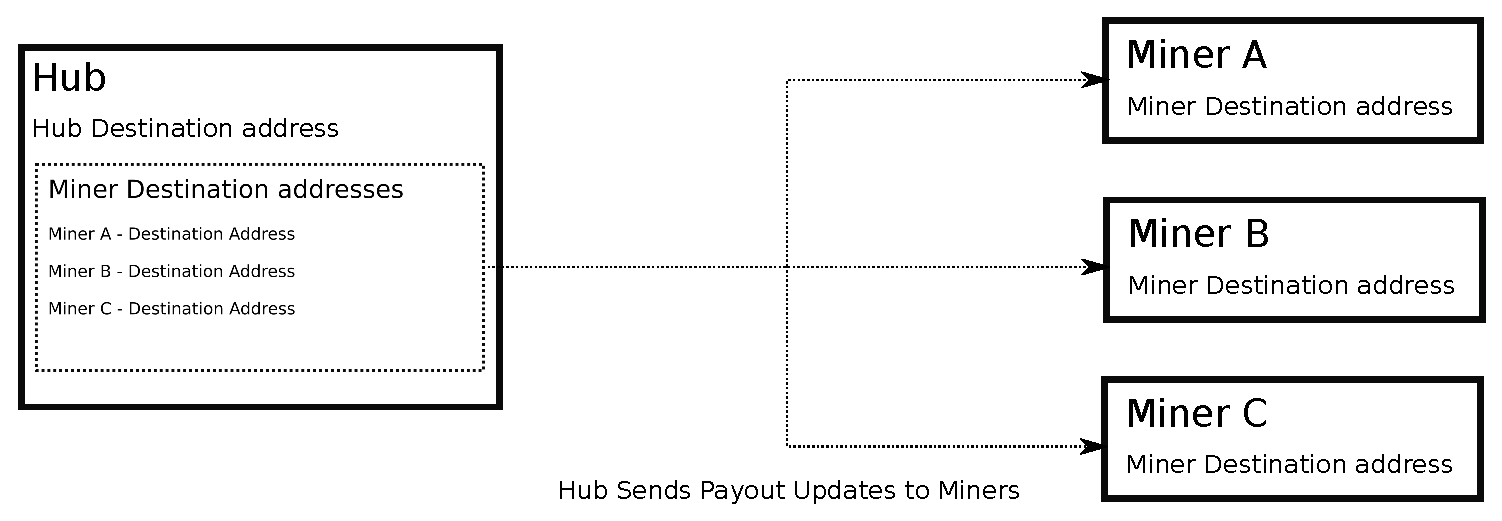
\includegraphics[width=0.8\textwidth]{payout-communication.eps}
    \caption{Hub sends one way updates to miners without revealing its
      destination address.}\label{fig:new-miner-communication}
  \end{center}
\end{figure}

There are two types of control messages exchanged between the hub and
the miner: 
\begin{enumerate*}
\item the channel creation messages when the miner first joins the
  pool and
\item the payout messages whenever a block is found.
\end{enumerate*}

Miners will run an I2P node next to their mining controller and setup
an incoming tunnel. Once the tunnel is ready, miners include their I2P
destination address in their share headers. The hub can then send
messages to the miner through the I2P tunnel. By hiding their real
I.P. address miners can increase their anonymity, and in turn help the
hub maintain its anonymity too.

The hub participates in the shares broadcast p2p network and
identifies a new miner along with the new miner's destination
address. Once the miner has mined for a certain time period, the hub
contacts the miner and provides its own destination address in the
message~\cite{i2p-streaming-library}. Figure~\ref{fig:new-miner-communication}
shows how the ``Miner A'' announces its I2P destination address,
enabling the hub to contact the miner for exchanging channel creation
messages.

To prevent the tunnel endpoint and gateway from seeing the messages
being exchanged, the hub and the miner use I2P's layered encryption,
called garlic routing~\cite{i2p-garlic-routing}. With the destination
addresses of both the new miner and the hub known to each other the
two can proceed to anonymously setup a payment channel as described in
Section~\ref{ref:channels}.

To send payouts as channel state updates, the hub again uses the I2P
destination address of each miner and sends a one way message, with no
reply destination included in the message. This allows the hub to
remain anonymous and makes it relatively hard to DDoS the hub. The hub
sends all miners updates to all payment channels. This allows the miner
who discovered a block to verify that the hub has paid everyone.

\section{Future Work}

The proposal presents an approach to enable decentralised mining for
bitcoin. Apart from the work of describing the various components in
detail, we also want to provide results from simulations, formalised
proofs of rewards schemes and possible extensions to using multiple
hubs.

Before we work on implementing they system, our next step is to
simulate p2p mining network using ns-3~\cite{ns3} and make informed
decisions about how large a network a single hub can support. The
observations we want to make are how large a p2p network can be
sustained without an increase in work lost by miners. Each hub and p2p
network can grow as long as miners are communicate WORK and SHARES
with each other with bounded latency and can limit their lost
work. With a simulation we want to find out the bounds of these.

We want to specify the p2p protocols and the message formats for both
the \textsc{share}s propagation and Channel management networks. By
publishing the specifications separate from the source code, we aim to
receive more feedback from the community. We want to use the model
presented in~\cite{incentives-compatible} to provide proofs for how
the rewards distribution is incentives compatible. We would like to
build further on the multiple hubs construction described by Belcher
once Taproot is activated on bitcoin.

\section{Acknowledgements}

Please to review! Many wow! ;)

\bibliography{proposal} 
\bibliographystyle{acm}

\end{document}
